% !TeX spellcheck = en_GB

\chapter{Assessment of \gls{tmf} Performance in Marine Environments}
\label{ch:comms_trust}
\lhead{Chapter \thechapter. \emph{\nameref{ch:comms_trust}}}

\section{\glspl{uan} as \gls{manet} analogue}


As \glspl{manet} grow beyond the terrestrial arena, their operation and the protocols designed around them must be reviewed to assess their suitability to different communications environments to ensure their continued security, reliability, and performance.
With demand for smaller, more decentralised \gls{manet} systems in a range of domains and applications, as well as a drive towards lower per-unit cost in all areas, \glspl{tmf} are increasingly applied to resource constrained applications, as the benefits and efficiencies these systems present are significant.
Many \glspl{uan} use \gls{manet} architectures, however the marine environment presents new challenges for trust management frameworks that have been developed for use in conventional (i.e. Terrestrial RF) \glspl{manet}.
These increasingly decentralised applications present unique threats against trust management \cite{Caiti2011}.

Previous research has established the advantages of implementing \glspl{tmf} in 802.11 based \glspl{manet}, particularly in terms of preventing selfish operation in collaborative systems \cite{Li2007}, and maintaining throughput in the presence of malicious actors \cite{Buchegger2002}

To date this work has been limited to terrestrial, RF based networks, which, as discussed in \autoref{ch:maritime_background}, is a much more favourable communications environment compared to the marine environment of \glspl{uan}, where extreme communications challenges are present (propagation delays, frequency dependent attenuation, fast and slow fading, refractive multipath distortion, etc.).
As a result of these challenges, in underwater environments, communications is both sparse and noisy.
That is to say that long delays create high susceptibility to contention blocking, requiring relatively low channel occupancy and significant back-offs and significant retransmission penalties in the face of a multitude of noise sources over inconsistent, non-linear, multi path transmissions.
Therefore the observations about the communications processes that are used to generate the trust metrics, occur much less frequently, with much greater error (noise) and delay than is experienced in terrestrial RF \glspl{manet}.
Beyond the constraints of the communications environment, knock on pressures in battery capacity, on-board processing, and locomotion simultaneously present opportunities and incentives for malicious or selfish actors to appear to cooperate while not reciprocating, in order to conserve power for instance.
These multiple aspects of potential incentives, trust, and fairness do not directly fall under the scope of single metric trusts discussed previously in \autoref{sec:tmfs}, and this context indicates that a multi-metric approach may be more appropriate.

As such, the use of trust methods developed in the terrestrial \gls{manet} space must be re-appraised for application within the underwater context \cite{Pavan2015}.

This chapter is primarily concerned with the analytical establishment of hard trust within a topologically dynamic network of mobile autonomous actors.
It is shown that single metric trust systems are not directly suitable for the marine context in terms of the different threat and cost scenario in that environment.
These single metric \glspl{tmf} provide malicious actors with a significant advantage if their activity does not impact that metric.

In the case where the attacker can subvert the \gls{tmf}, the metric under assessment by that \gls{tmf} does not cover the threat mounted by the attacker.
This causes a significant negative effect on the efficiency of the network, as the \gls{tmf} is assumed to have reduced the possible set of attacks when it has actually made it more advantageous to attack a different part of the networks operation.
An example of such a situation would be in a \gls{tmf} focused on \gls{plr} where an attacker selectively delays packets going through it, reducing overall throughput but not dropping any packets.
Such behaviour would not be detected by the \gls{tmf}.

For the purposes of this work, from those \glspl{tmf} discussed in~\autoref{sec:tmfs}, Hermes trust establishment, \gls{otmf} and \gls{mtfm} are selected as indicative single and multi metrics frameworks for comparison, as Hermes captures the core operation of a pure single metric assessment methodology and \gls{otmf} provides a comparison that combines assessments from across nodes to develop trust opinions.
\gls{mtfm} is also included as an example of an existing multi-metric \gls{tmf} that looking purely at the communications domain.


\section{Modelling of \gls{uan} network}\label{sec:initialsystemcharacterization}

\subsection{Mobility, Topology, and Communications}

Four mobility patterns are investigated:
\begin{enumerate}
	\item All Nodes Static
	\item Malicious node mobile
	\item Malicious node mobile, all other nodes static
	\item All nodes mobile
\end{enumerate}

For this case, the mobility model used is a random walk on the nodes modelled kinematic response, i.e.\ the node periodically picks a spherically normalised random direction in the XY plane.
Maximum node speed (limited by kinematic acceleration/turning constraints) is 1.5$ms^{-1}$\cite{Milgram2001}.

The six nodes are initially arranged as per Fig.~\ref{fig:s1_layout} with each node on average $\SI{100}{\meter}$ from each other as per \cite{Guo11}.
The use of six nodes and the particular layout enables the investigation of the three trust relationships based on minimum path topologies, such that the node generating the trust assessments, $n_0$ has Direct, Recommendation, and Indirect trust assessments of $n_1$ available to it from itself, $[n_2,n_3]$, and $[n_4,n_5]$ respectively. 
(See Section~\ref{sec:trust_topologies})

Collaborations with NATO \gls{cmre} in La Spezia, and \glspl{dstl} Naval Systems Group inform that this is a practical team-size for environmental and defence applications.
%
\begin{figure}[h]
	\centering
	\begin{tikzpicture}[auto, node distance=1.5cm and 0.5cm, line width=2pt, >=latex', baseline=(a.base)]
	\node [sum] (n0) {$n_0$};
	\node [sum, right =of n0] (n1) {$n_1$};
	\node [sum, above right =of n0] (n2) {$n_2$};
	\node [sum, below right =of n0] (n3) {$n_3$};
	\node [sum, above right =of n1, xshift=10,yshift=-15] (n4) {$n_4$};
	\node [sum, below right =of n1, xshift=10,yshift=15](n5) {$n_5$};
	
	
	\draw (n0) -- (n1);
	\draw (n0) -- (n2);	
	\draw (n0) -- (n3);

	\draw (n1) -- (n2);	
	\draw (n1) -- (n3);
	\draw (n1) -- (n4);
	\draw (n1) -- (n5);	
	
	\draw (n2) -- (n4);
	
	\draw (n3) -- (n5);
	
	\draw (n4) -- (n5);
	
	\end{tikzpicture}
	\caption{Initial layout with nodes spaced an average of \SI{100}{\meter} apart}
	\label{fig:s1_layout}
\end{figure}
%

\subsubsection{Simulation Background}

Simulations were conducted using a Python based simulation framework, SimPy \cite{Mueller2003SimPy}, with a network stack built upon \gls{auv}NetSim \cite{Miquel2008}, with transmission parameters (\autoref{tab:sysconstraints}) taken from and validated against existing studied \cite{Stojanovic2007,Stefanov2011,Sehgal2010}

Given the differences in delay and propagation between RF and marine networks, it would not be expected that the same application rates (e.g.\ packet emission rates or throughput) and node separations are equally stable in this environment.
Therefore, a zone of performance is characterised within which the network has stable operation.
%
\begin{table}[h]
	\caption{Comparison of system model constraints as applied between Terrestrial and Marine communications} \label{tab:sysconstraints}
	\begin{center}
		\setlength{\tabcolsep}{8pt}
		\begin{tabular}{lccc}
			\toprule
			Parameter & Terrestrial & Marine \\
			\midrule
			Simulated Duration & \SI{300}{\second} & \SI{18000}{\second}\\
			Trust Sampling Period & \SI{1}{\second} & \SI{600}{\second} \\
			Simulated Area & \SI{0.7}{\kilo\meter\squared} & \SIrange{0.7}{4}{\kilo\meter\squared} \\
			Transmission Range & \SI{0.25}{\kilo\meter} & \SI{1.5}{\kilo\meter} \\
			Physical Layer & RF(802.11) & Acoustic\\
			Propagation Speed&  \SI{3e8}{\meter\per\second} & \SI{1490}{\meter\per\second}\\
			Center Frequency & \SI{2.6e9}{\hertz} & \SI{2e4}{\hertz} \\
			Bandwidth& \SI{22e6}{\hertz} & \SI{1e4}{\hertz}\\
			MAC Type & CSMA/DCF & CSMA/CA\\
			Routing Protocol & DSDV & FBR \\
			Max Speed & \SI{5}{\meter\per\second} & \SI{1.5}{\meter\per\second} \\
			Max Data Rate & \SI{5e6}{\bit\per\second} & $\approx\SI{240}{\bit\per\second}$ \\
			Packet Size & \SI{4096}{\bit} & \SI{9600}{\bit} \\
			Single Transmission Duration & \SI{10}{\second} & \SI{32}{\second} \\
			Single Transmission Size & \SI{1e7}{\bit} & \SI{9600}{\bit} \\
			\bottomrule
		\end{tabular}
		\setlength{\tabcolsep}{6pt}
	\end{center}
\end{table}
%


\subsection{Establishing Scale Factors in Communications Rate}

In this section the simulated communications environment is characterised to establish an optimal packet emission rate for comparison against \cite{Guo11}.
This optimal emission rate is taken to be an emission rate that provides reasonable network stability and protection from network saturation.
Network saturation is the point at which a network can no longer successfully deliver the offered load\footnote{It will become important to note that Offered Load in this case includes packet retransmissions} presented to it to the relevant destinations (throughput), and is characterised by a peak and a subsequent decline in the throughput of the network when varying the packet emission rate. 

Formally, this saturation rate occurs if

\begin{equation}
N\lambda_s>\mu_\text{max}
\end{equation}

\todo{ADD NEXT: Attempt to Formalise the relationship between separation, offered load, throughput and delay using Bianchi Model \cite{Manshaei2007}}

In order to establish the point at which the network becomes saturated due, a range of packet emission rates were explored between 0.01 packets per second (pps), equivalent to 96 bits of offered load per node, up to $0.07 pps$ ($672 bps$ per node).
Initial node separation was set as per \citet{Guo11} at $\SI{100}{\meter}$, and each simulation is run 16 times, with each instance modelling a 8 hour mission time.
This configuration and duration are specified to correlate to previously discussed mobile collaborative port protection scenarios from \autoref{sec:marine_ops}.

Looking first at the Static mobility case, where all nodes are stationary; from~\autoref{fig:emission_throughput_performance_bella_static} it is already clear that the throughput curve, exhibits a saturation point close to 0.025 pps.
Similarly in~\autoref{fig:emission_prod_breakdown_bella_static}, the precipitous drop in packet delivery probability beyond 0.025 pps, indicating that this is a strong candidate value for an upper-limit to the safe operating zone in terms of packet emission in the small static case.
From~\autoref{fig:emission_delay_variation_bella_static}, raising packet emissions above $0.25pps$ results in a significant increase in end-to-end delay.
As per~\autoref{tab:sysconstraints}, the \gls{csma} based \gls{mac} incurs a certain amount of control overhead in the form of \gls{rts} packets, when a node attempts to acquire time in its neighbourhood.
In~\autoref{fig:emission_rts_ratio_bella_static}, the ratio of Control/Data packets increases linearly up to 1.5 until just before $0.025pps$, and then accelerates to almost 2.5, further demonstrating that the network has become critically congested.
It is worthwhile noting that in~\autoref{fig:emission_throughput_performance_bella_static} that even as the saturation point is passed, packet collisions do not significantly increase, and that the saturation is in fact driven by contention in the medium rather than congestion-collisions.

Results are also included from the remaining mobility cases (all nodes mobile; all-but-one node mobile; single mobile node), however from Figs.~\ref{fig:emission_all},~ \ref{fig:emission_bella_all_mobile}-~\ref{fig:emission_bella_single_mobile} that the throughput threshold behaviour is qualitatively similar regardless of mobility for this initial node separation.



\begin{figure}[h]
	\begin{subfigure}[t]{0.5\textwidth}
		\centering
		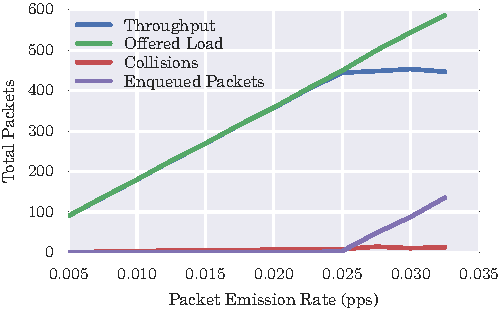
\includegraphics[width=\textwidth]{emission_throughput_performance_bella_static}
		\caption{Static}
		\label{fig:emission_throughput_performance_sum_bella_static}
	\end{subfigure}
	\begin{subfigure}[t]{0.5\textwidth}
		\centering
		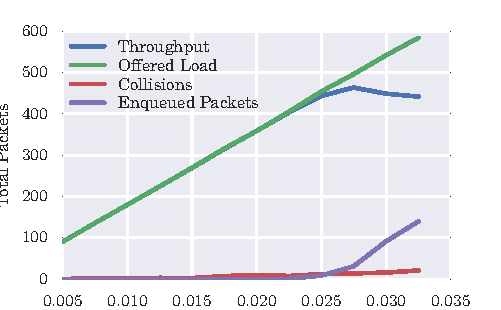
\includegraphics[width=\textwidth]{emission_throughput_performance_bella_all_mobile}
		\caption{All Mobile}
		\label{fig:emission_throughput_performance_sum_bella_all_mobile}
	\end{subfigure}  
	
	\begin{subfigure}[t]{0.5\textwidth}
		\centering
		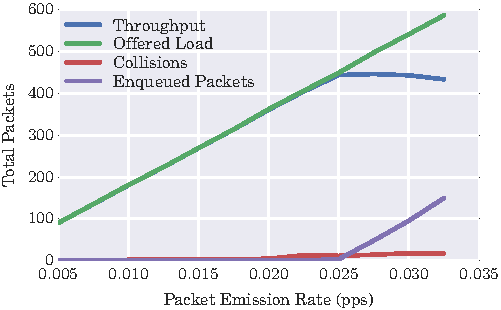
\includegraphics[width=\textwidth]{emission_throughput_performance_bella_allbut1_mobile}
		\caption{All-but-one Mobile}
		\label{fig:emission_throughput_performance_sum_bella_allbut1_mobile}
	\end{subfigure}  
	\begin{subfigure}[t]{0.5\textwidth}
		\centering
		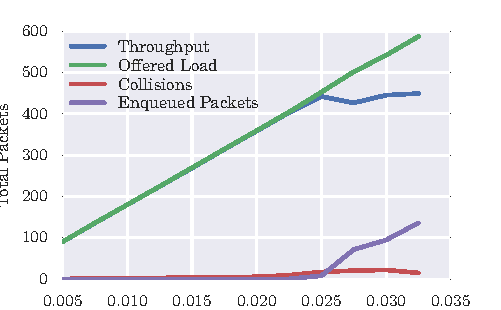
\includegraphics[width=\textwidth]{emission_throughput_performance_bella_single_mobile}
		\caption{Single Mobile}
		\label{fig:emission_throughput_performance_sum_bella_single_mobile}
	\end{subfigure}
	\caption{Throughput performance overview for all mobilities under varying emission rates}
	\label{fig:emission_all}
\end{figure}


\begin{figure}[tp!]
	\begin{subfigure}[t]{0.5\textwidth}
		\centering
		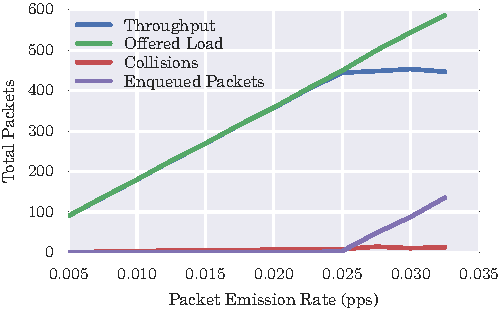
\includegraphics[width=\textwidth]{emission_throughput_performance_bella_static}
		\caption{Packet delivery}
		\label{fig:emission_throughput_performance_bella_static}
	\end{subfigure}
	%
	\begin{subfigure}[t]{0.5\textwidth}
		\centering
		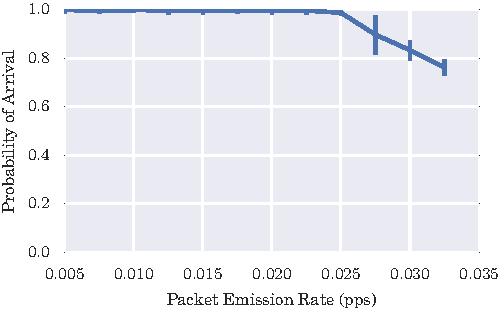
\includegraphics[width=\textwidth]{emission_prod_breakdown_bella_static}
		\caption{Probability of arrival}
		\label{fig:emission_prod_breakdown_bella_static}
	\end{subfigure}
	
	\begin{subfigure}[t]{0.5\textwidth}
		\centering
		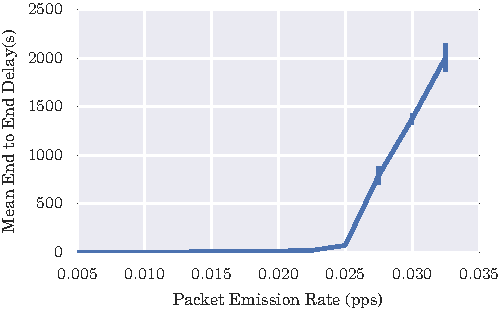
\includegraphics[width=\textwidth]{emission_delay_variation_bella_static}
		\caption{End-to-end delay}
		\label{fig:emission_delay_variation_bella_static}
	\end{subfigure}
	%
	\begin{subfigure}[t]{0.5\textwidth}
		\centering
		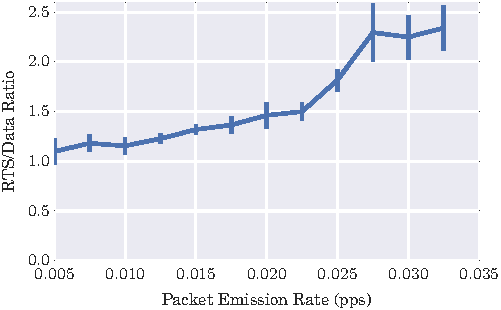
\includegraphics[width=\textwidth]{emission_rts_ratio_bella_static}
		\caption{RTS Ratios}
		\label{fig:emission_rts_ratio_bella_static}
	\end{subfigure}
	\caption{Network performance varying packet emission rates for the static case}
	\label{fig:emission_bella_static}
\end{figure}


\begin{figure}[bp!]
	\begin{subfigure}[t]{0.5\textwidth}
		\centering
		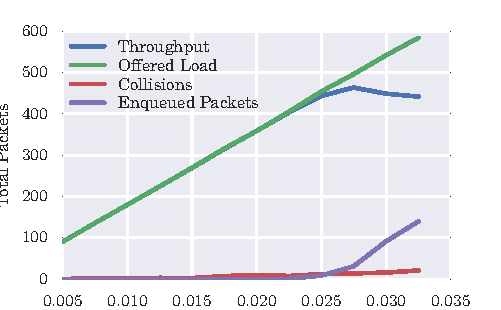
\includegraphics[width=\textwidth]{emission_throughput_performance_bella_all_mobile}
		\caption{Packet delivery}
		\label{fig:emission_throughput_performance_bella_all_mobile}
	\end{subfigure}
	%
	\begin{subfigure}[t]{0.5\textwidth}
		\centering
		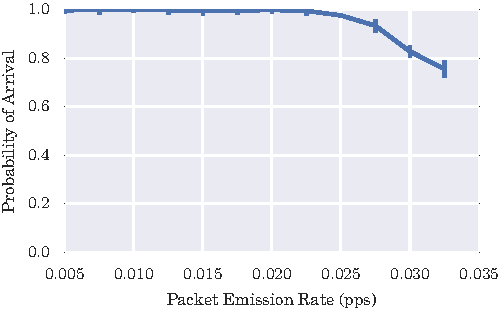
\includegraphics[width=\textwidth]{emission_prod_breakdown_bella_all_mobile}
		\caption{Probability of arrival}
		\label{fig:emission_prod_breakdown_bella_all_mobile}
	\end{subfigure}
	
	\begin{subfigure}[t]{0.5\textwidth}
		\centering
		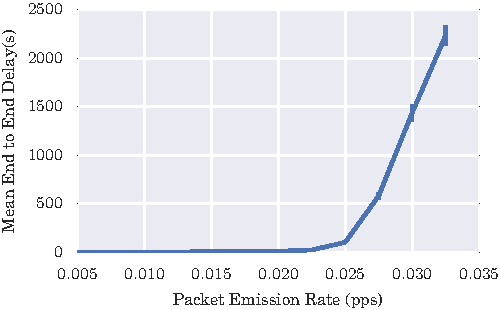
\includegraphics[width=\textwidth]{emission_delay_variation_bella_all_mobile}
		\caption{End-to-end delay}
		\label{fig:emission_delay_variation_bella_all_mobile}
	\end{subfigure}
	%
	\begin{subfigure}[t]{0.5\textwidth}
		\centering
		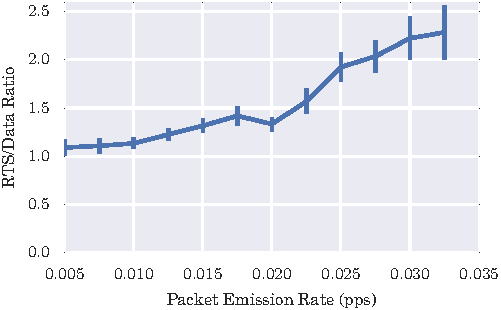
\includegraphics[width=\textwidth]{emission_rts_ratio_bella_all_mobile}
		\caption{RTS Ratios}
		\label{fig:emission_rts_ratio_bella_all_mobile}
	\end{subfigure}
	\caption{Network performance varying packet emission rates for the all mobile case}
	\label{fig:emission_bella_all_mobile}
\end{figure}


\begin{figure}[tp!]
	\begin{subfigure}[t]{0.5\textwidth}
		\centering
		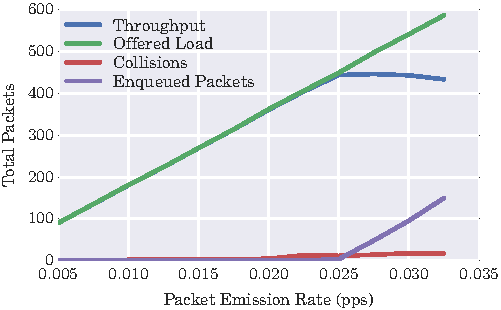
\includegraphics[width=\textwidth]{emission_throughput_performance_bella_allbut1_mobile}
		\caption{Packet delivery}
		\label{fig:emission_throughput_performance_bella_allbut1_mobile}
	\end{subfigure}
	%
	\begin{subfigure}[t]{0.5\textwidth}
		\centering
		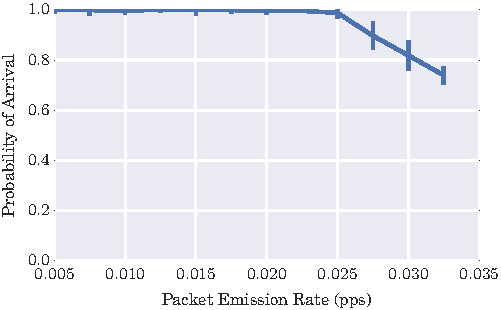
\includegraphics[width=\textwidth]{emission_prod_breakdown_bella_allbut1_mobile}
		\caption{Probability of arrival}
		\label{fig:emission_prod_breakdown_bella_allbut1_mobile}
	\end{subfigure}
	
	\begin{subfigure}[t]{0.5\textwidth}
		\centering
		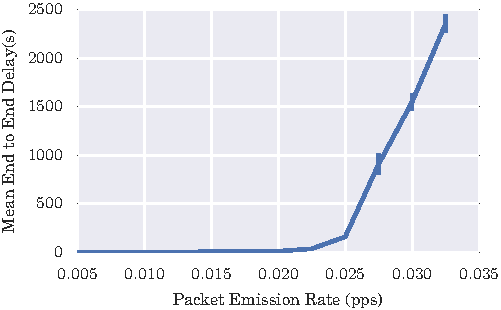
\includegraphics[width=\textwidth]{emission_delay_variation_bella_allbut1_mobile}
		\caption{End-to-end delay}
		\label{fig:emission_delay_variation_bella_allbut1_mobile}
	\end{subfigure}
	%
	\begin{subfigure}[t]{0.5\textwidth}
		\centering
		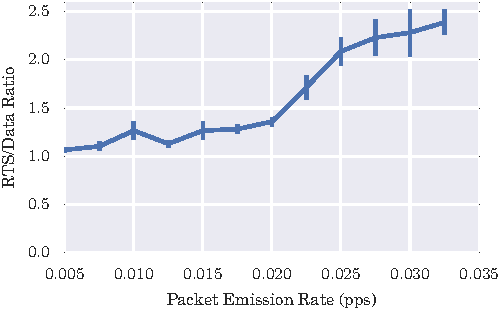
\includegraphics[width=\textwidth]{emission_rts_ratio_bella_allbut1_mobile}
		\caption{RTS Ratios}
		\label{fig:emission_rts_ratio_bella_allbut1_mobile}
	\end{subfigure}
	\caption{Network performance varying packet emission rates for the all-but-one mobile case}
	\label{fig:emission_bella_allbut1_mobile}
\end{figure}

\begin{figure}[bp!]
	\begin{subfigure}[t]{0.5\textwidth}
		\centering
		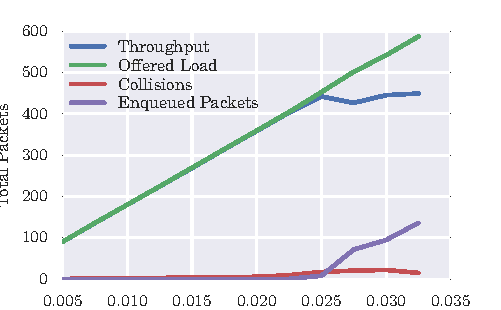
\includegraphics[width=\textwidth]{emission_throughput_performance_bella_single_mobile}
		\caption{Packet delivery}
		\label{fig:emission_throughput_performance_bella_single_mobile}
	\end{subfigure}
	%
	\begin{subfigure}[t]{0.5\textwidth}
		\centering
		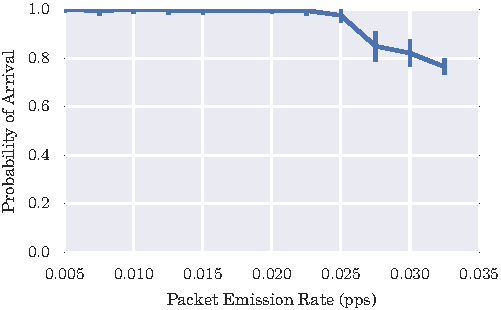
\includegraphics[width=\textwidth]{emission_prod_breakdown_bella_single_mobile}
		\caption{Probability of arrival}
		\label{fig:emission_prod_breakdown_bella_single_mobile}
	\end{subfigure}
	
	\begin{subfigure}[t]{0.5\textwidth}
		\centering
		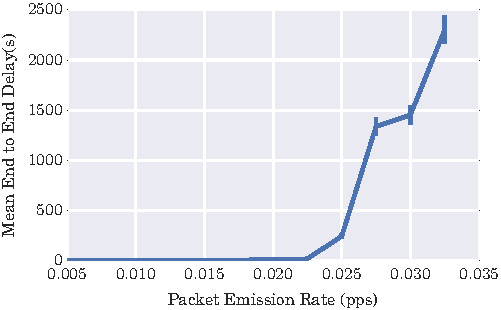
\includegraphics[width=\textwidth]{emission_delay_variation_bella_single_mobile}
		\caption{End-to-end delay}
		\label{fig:emission_delay_variation_bella_single_mobile}
	\end{subfigure}
	%
	\begin{subfigure}[t]{0.5\textwidth}
		\centering
		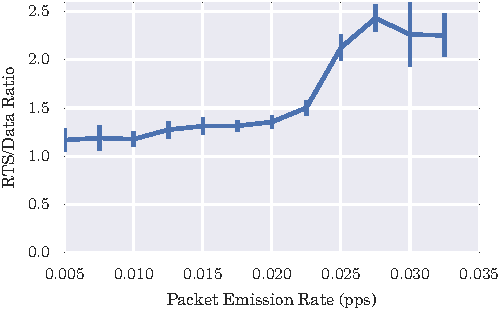
\includegraphics[width=\textwidth]{emission_rts_ratio_bella_single_mobile}
		\caption{RTS Ratios}
		\label{fig:emission_rts_ratio_bella_single_mobile}
	\end{subfigure}
	\caption{Network performance varying packet emission rates for the single mobile case}
	\label{fig:emission_bella_single_mobile}
\end{figure}

\clearpage

\subsection{Scale Factors in Physical Node Distribution}

In this section the effect of node-separation scaling on communications operation is characterised for comparison against \cite{Guo11}. 
This is particularly important considering the significant scale factor differences in terms of the speed of propagation in the medium, and the range of potential desired operation.

From~\autoref{tab:sysconstraints}, the operating transmission range of acoustic is $\approx 6$ times further than 802.11, indicating that a suitable operating environment will have an area $\approx \sqrt{6}$ times the area of the 802.11 case. Therefore, a reasonable experimental range would have an upper bound of performance around this scaling factor, where nodes are approximately 400$m$ apart. 

According to \citet{Xu2002}, \gls{rts}/\gls{cts} handshake functionality cannot operate well as interference protection at node separations beyond 0.56 times the transmission range\cite{Xu2002}.
In the case of marine acoustic transmission at the stated power output, above $\SI{1500}{\meter} \times 0.56 = \SI{840}{\meter}$, handshake overheads should begin to dominate channel access.\todo{FIX CODE:redo these graphs with wider separations ~ \SI{1000}{\meter}}
This is due to reduced channel availability due to collisions, which are then due to a much longer potential contention period between nodes. 

A reasonable range around this is to scale from 100$m$ apart on average to $\SI{800}{\meter}$, and from the previous section, a packet emission rate of $0.02pps$ (slightly below the $0.025pps$ saturation threshold) is used to explore this space.
The ``environment'' of the simulations is also scaled in accordance with the node scaling, based on an initial environmental ``water-box'' of $\SI{1}{\kilo\meter}$ for the $\SI{100}{\meter}$ node separation, i.e.\ the water-box is consistently ten times larger than the initial node separation.

In the case where all nodes remain static, increasing node separation does not significantly impact throughput, delay, delivery probability or \gls{rts} ratios until rising above 700$m$ (Fig.~\ref{fig:separation_bella_static}), nearly double our initial estimate of where an appropriate separation zone would be.

The other mobility cases tell a very different story; as can be seen in~\autoref{fig:separation_throughput_performance_sum_bella_single_mobile}, where adding a single mobile node to the network induces a saturation-style response at 500$m$, and this drops further in~\autoref{fig:separation_throughput_performance_sum_bella_allbut1_mobile} and~\autoref{fig:separation_throughput_performance_sum_bella_all_mobile}, reducing the separation of saturation at this emission rate to just 300$m$.

Another aspect of these results to highlight is that the Offered Load presented to the network \emph{increases} beyond the collapse of the throughput curve. 
This indicates that there is a subtly different saturation behaviour with respect to separation than the simple congestion argument with respect to packet emission rate; packets are simply taking too long to cross the increasingly sparse network and in-transit packet routes are logically disconnected and require retransmission.



\subsection{Combined Scale Factor Analysis}
\begin{figure}[h]
	\begin{subfigure}[t]{0.5\textwidth}
		\centering
		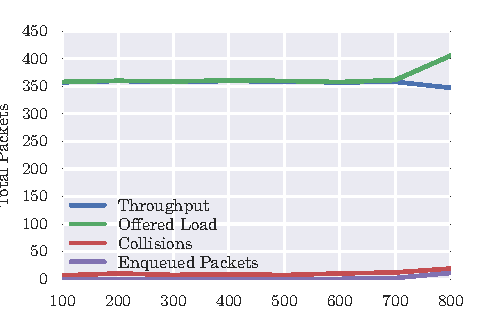
\includegraphics[width=\textwidth]{separation_throughput_performance_bella_static}
		\caption{Static}
		\label{fig:separation_throughput_performance_sum_bella_static}
	\end{subfigure}
	\begin{subfigure}[t]{0.5\textwidth}
		\centering
		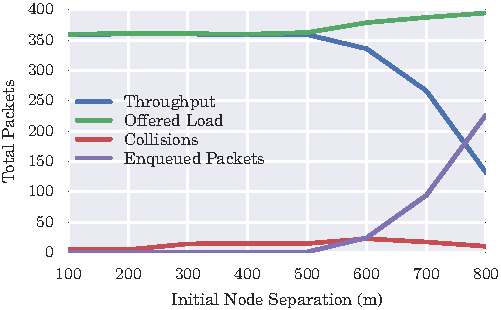
\includegraphics[width=\textwidth]{separation_throughput_performance_bella_single_mobile}
		\caption{Single Mobile}
		\label{fig:separation_throughput_performance_sum_bella_single_mobile}
	\end{subfigure}
	
	\begin{subfigure}[t]{0.5\textwidth}
		\centering
		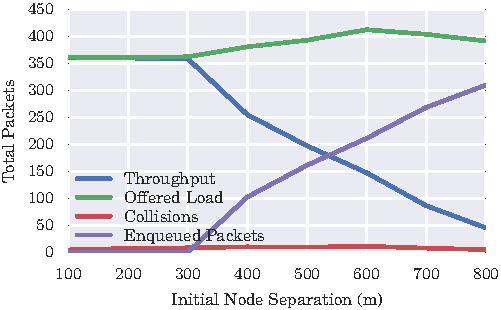
\includegraphics[width=\textwidth]{separation_throughput_performance_bella_allbut1_mobile}
		\caption{All-but-one Mobile}
		\label{fig:separation_throughput_performance_sum_bella_allbut1_mobile}
	\end{subfigure}  
	\begin{subfigure}[t]{0.5\textwidth}
		\centering
		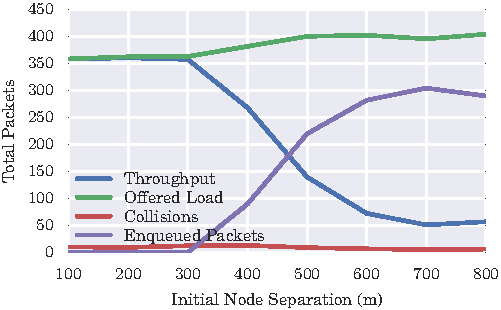
\includegraphics[width=\textwidth]{separation_throughput_performance_bella_all_mobile}
		\caption{All Mobile}
		\label{fig:separation_throughput_performance_sum_bella_all_mobile}
	\end{subfigure}  
	\caption{Throughput performance overview for all mobilities under varying separation}
	\label{fig:separation_all}
\end{figure}

% These figures should be colocated
\begin{figure}[tp!]
	\begin{subfigure}[t]{0.5\textwidth}
		\centering
		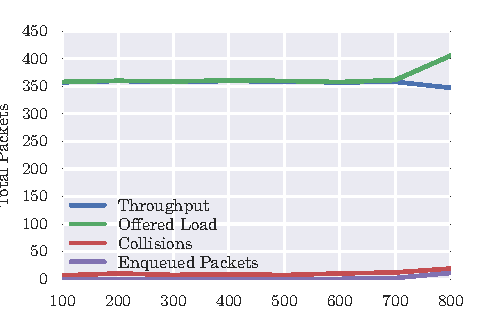
\includegraphics[width=\textwidth]{separation_throughput_performance_bella_static}
		\caption{Packet delivery}
		\label{fig:separation_throughput_performance_bella_static}
	\end{subfigure}
	%
	\begin{subfigure}[t]{0.5\textwidth}
		\centering
		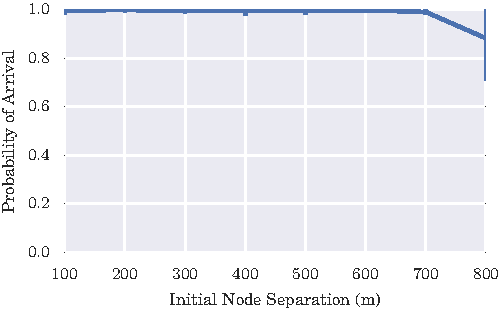
\includegraphics[width=\textwidth]{separation_prod_breakdown_bella_static}
		\caption{Probability of arrival}
		\label{fig:separation_prod_breakdown_bella_static}
	\end{subfigure}
	
	\begin{subfigure}[t]{0.5\textwidth}
		\centering
		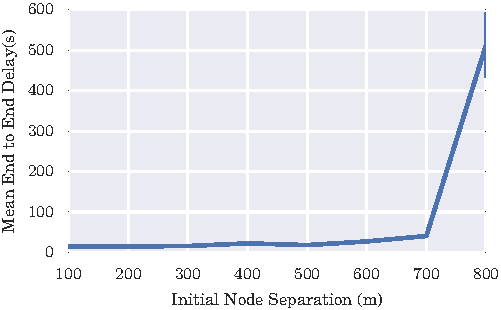
\includegraphics[width=\textwidth]{separation_delay_variation_bella_static}
		\caption{End-to-end delay}
		\label{fig:separation_delay_variation_bella_static}
	\end{subfigure}
	%
	\begin{subfigure}[t]{0.5\textwidth}
		\centering
		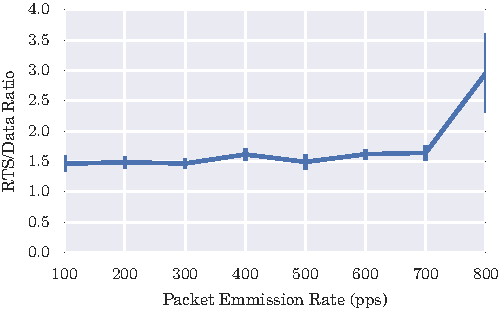
\includegraphics[width=\textwidth]{separation_rts_ratio_bella_static}
		\caption{RTS Ratios}
		\label{fig:separation_rts_ratio_bella_static}
	\end{subfigure}
	\caption{Network performance varying node separation for the static case}
	\label{fig:separation_bella_static}
\end{figure}


\begin{figure}[bp!]
	\begin{subfigure}[t]{0.5\textwidth}
		\centering
		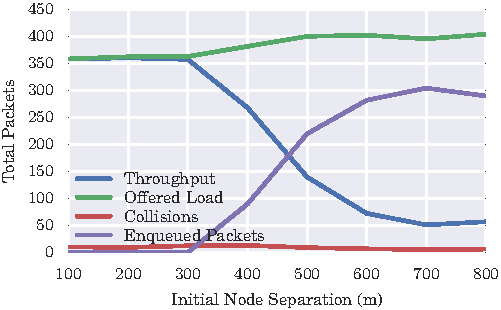
\includegraphics[width=\textwidth]{separation_throughput_performance_bella_all_mobile}
		\caption{Packet delivery}
		\label{fig:separation_throughput_performance_bella_all_mobile}
	\end{subfigure}
	%
	\begin{subfigure}[t]{0.5\textwidth}
		\centering
		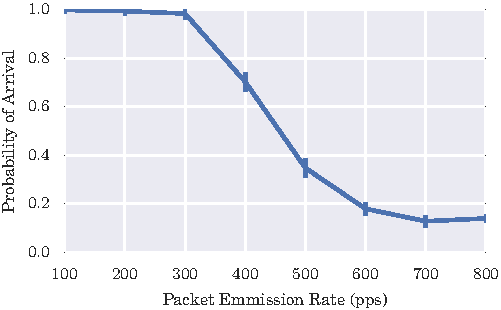
\includegraphics[width=\textwidth]{separation_prod_breakdown_bella_all_mobile}
		\caption{Probability of arrival}
		\label{fig:separation_prod_breakdown_bella_all_mobile}
	\end{subfigure}
	
	\begin{subfigure}[t]{0.5\textwidth}
		\centering
		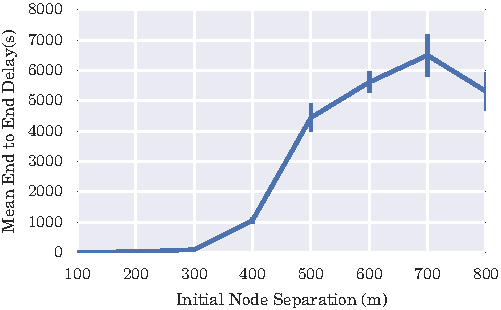
\includegraphics[width=\textwidth]{separation_delay_variation_bella_all_mobile}
		\caption{End-to-end delay}
		\label{fig:separation_delay_variation_bella_all_mobile}
	\end{subfigure}
	%
	\begin{subfigure}[t]{0.5\textwidth}
		\centering
		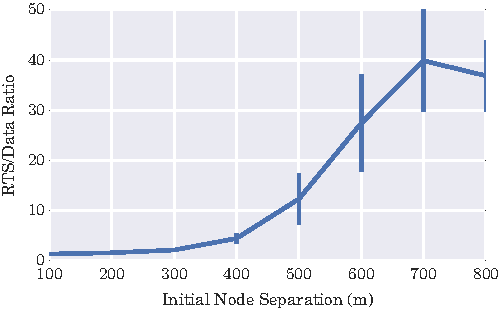
\includegraphics[width=\textwidth]{separation_rts_ratio_bella_all_mobile}
		\caption{RTS Ratios}
		\label{fig:separation_rts_ratio_bella_all_mobile}
	\end{subfigure}
	\caption{Network performance varying node separation for the all mobile case}
	\label{fig:separation_bella_all_mobile}
\end{figure}


\begin{figure}[tp!]
	\begin{subfigure}[t]{0.5\textwidth}
		\centering
		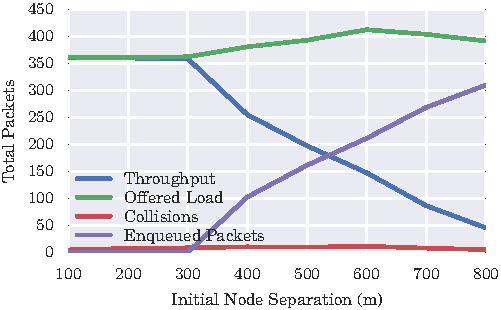
\includegraphics[width=\textwidth]{separation_throughput_performance_bella_allbut1_mobile}
		\caption{Packet delivery}
		\label{fig:separation_throughput_performance_bella_allbut1_mobile}
	\end{subfigure}
	%
	\begin{subfigure}[t]{0.5\textwidth}
		\centering
		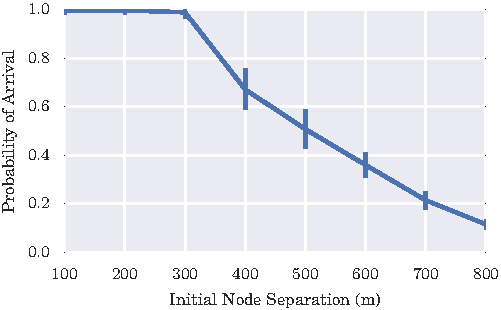
\includegraphics[width=\textwidth]{separation_prod_breakdown_bella_allbut1_mobile}
		\caption{Probability of arrival}
		\label{fig:separation_prod_breakdown_bella_allbut1_mobile}
	\end{subfigure}
	
	\begin{subfigure}[t]{0.5\textwidth}
		\centering
		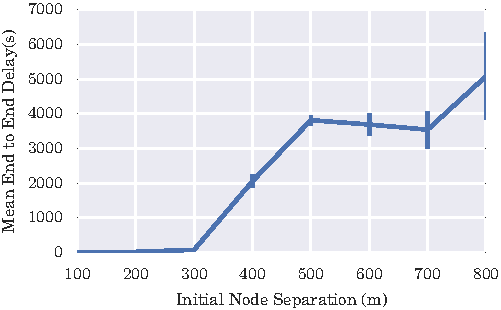
\includegraphics[width=\textwidth]{separation_delay_variation_bella_allbut1_mobile}
		\caption{End-to-end delay}
		\label{fig:separation_delay_variation_bella_allbut1_mobile}
	\end{subfigure}
	%
	\begin{subfigure}[t]{0.5\textwidth}
		\centering
		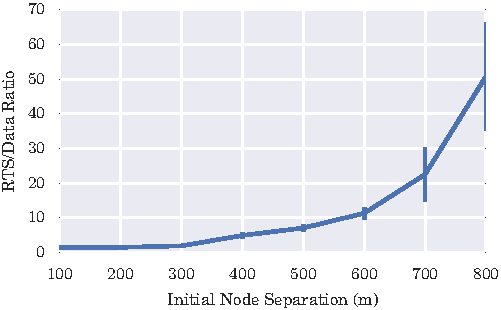
\includegraphics[width=\textwidth]{separation_rts_ratio_bella_allbut1_mobile}
		\caption{RTS Ratios}
		\label{fig:separation_rts_ratio_bella_allbut1_mobile}
	\end{subfigure}
	\caption{Network performance varying node separation for the all-but-one mobile case}
	\label{fig:separation_bella_allbut1_mobile}
\end{figure}

\begin{figure}[bp!]
	\begin{subfigure}[t]{0.5\textwidth}
		\centering
		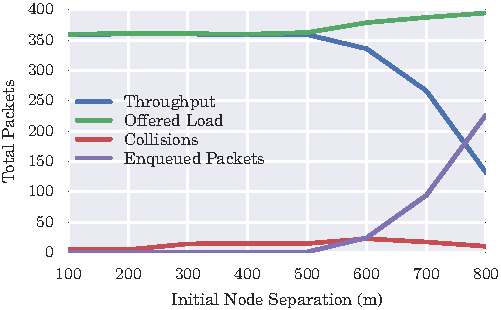
\includegraphics[width=\textwidth]{separation_throughput_performance_bella_single_mobile}
		\caption{Packet delivery}
		\label{fig:separation_throughput_performance_bella_single_mobile}
	\end{subfigure}
	%
	\begin{subfigure}[t]{0.5\textwidth}
		\centering
		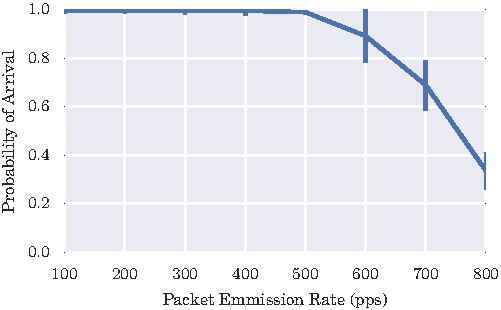
\includegraphics[width=\textwidth]{separation_prod_breakdown_bella_single_mobile}
		\caption{Probability of arrival}
		\label{fig:separation_prod_breakdown_bella_single_mobile}
	\end{subfigure}
	
	\begin{subfigure}[t]{0.5\textwidth}
		\centering
		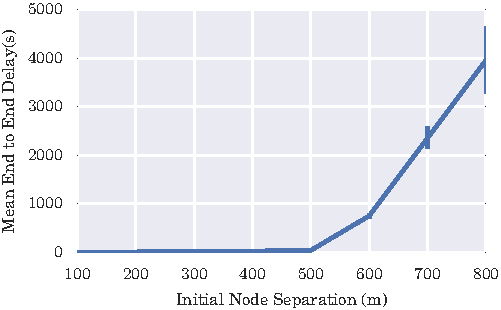
\includegraphics[width=\textwidth]{separation_delay_variation_bella_single_mobile}
		\caption{End-to-end delay}
		\label{fig:separation_delay_variation_bella_single_mobile}
	\end{subfigure}
	%
	\begin{subfigure}[t]{0.5\textwidth}
		\centering
		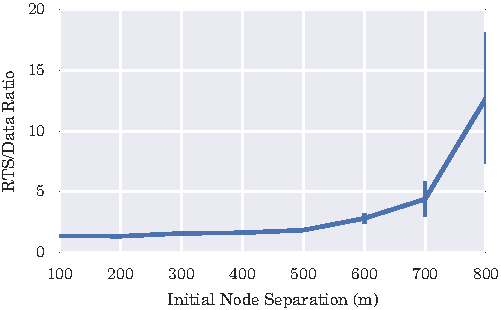
\includegraphics[width=\textwidth]{separation_rts_ratio_bella_single_mobile}
		\caption{RTS Ratios}
		\label{fig:separation_rts_ratio_bella_single_mobile}
	\end{subfigure}
	\caption{Network performance varying node separation for the single mobile case}
	\label{fig:separation_bella_single_mobile}
\end{figure}


% scripts.publication_scripts.test_Thesis_lazy.ThesisLazyDiagrams#test_PacketStatsGraphs
\begin{table}[h]
	\caption{Tabular view of data from~\autoref{fig:separation_bella_single_mobile}, including ideal propagation time} \label{tab:separation_bella_single_mobile}
	\begin{center}
		\hyphenpenalty 10000
		\begin{tabular}{
            *{2}{@{\hspace{1em}}r@{\hspace{1em}}}
            *{3}{@{\hspace{1em}}p{0.1\textwidth} @{\hspace{1em}}}  }
\toprule
 Initial Node Separation (m) &  Delay(s) &  Probability of Arrival &  RTS/Data Ratio &  Ideal Delivery Time(s) \\
\midrule
                         100 &   10.3551 &                  0.9977 &          1.3546 &                  1.0314 \\
                         200 &   11.1631 &                  0.9973 &          1.3322 &                  1.1029 \\
                         300 &   24.2225 &                  0.9983 &          1.5650 &                  1.1743 \\
                         400 &   29.4864 &                  0.9965 &          1.6210 &                  1.2457 \\
                         500 &   41.7093 &                  0.9904 &          1.8331 &                  1.3171 \\
                         600 &  753.4040 &                  0.8922 &          2.8038 &                  1.3886 \\
                         700 & 2360.0826 &                  0.6899 &          4.3889 &                  1.4600 \\
                         800 & 3963.9830 &                  0.3360 &         12.7323 &                  1.5314 \\
\bottomrule
\end{tabular}

	\end{center}
\end{table}


\clearpage





Its clear from the previous results that the relationship between emission rates, separations and mobilities is tightly coupled and not totally clear cut. 
To arrive at a more optimal operating region, a coupled analysis is performed across both emission rate and initial separation distance.

Given what has been discussed so far; it's clear that in identifying an appropriate operating region, it is important to not only ensure throughput, but that that throughput is timely.
For instance, in~\autoref{fig:separation_bella_single_mobile} (tabulated in~\autoref{tab:separation_bella_single_mobile}), a small increase in separation beyond the apparent throughput-peak at 500$m$ to 600$m$, which constitutes an increased ideal marine acoustic ``time of flight'' between nodes by 0.02$s$, increases the average actual delay by 1800\%. 

To capture these performance requirements, the feature scaled product of Throughput and Delay is taken and plotted against rate and separation in~\autoref{fig:2d_normed_product}.\todo[inline]{FIX: This does NOT make for easy comparison between graphs as the scaling is different for each mobility, but I need to think about how to fairly solve this}

\begin{equation}
V = |S] \times (1 - |D|)
\label{eq:normed_product}
\end{equation}

For each scenario, the observed Throughput across the network ($S$ in bytes) is normalised across all observations (i.e.\ each combination of Node Separation and Emission Rate), as is average end-to-end Delay ($D$). The normalised delay is inverted ($1-|D|$) and the product of this and the normalised throughput is used as the basis of a two-dimensional linear interpolation shown in \autoref{fig:2d_normed_product}.




\begin{figure}[h]
	\begin{subfigure}[t]{0.5\textwidth}
		\centering
		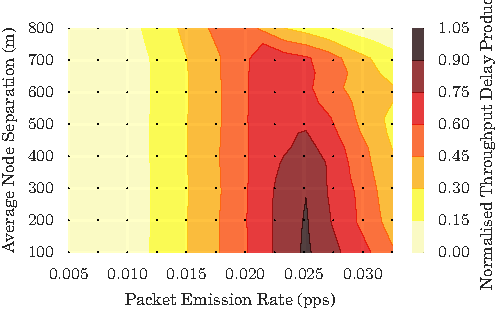
\includegraphics[width=\textwidth]{2d_normed_product_bella_static}
		\caption{Static}
		\label{fig:2d_normed_product_bella_static}
	\end{subfigure}
	\begin{subfigure}[t]{0.5\textwidth}
		\centering
		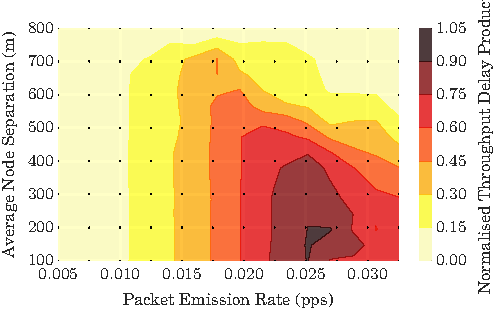
\includegraphics[width=\textwidth]{2d_normed_product_bella_single_mobile}
		\caption{Single Mobile}
		\label{fig:2d_normed_product_bella_single_mobile}
	\end{subfigure}
	
	\begin{subfigure}[t]{0.5\textwidth}
		\centering
		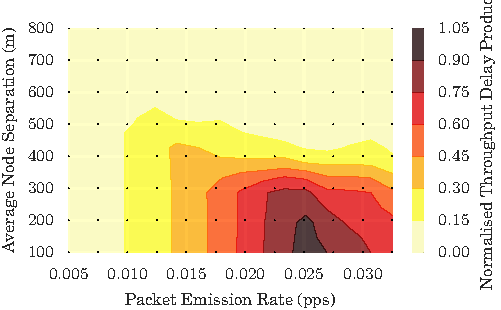
\includegraphics[width=\textwidth]{2d_normed_product_bella_allbut1_mobile}
		\caption{All-but-one Mobile}
		\label{fig:2d_normed_product_bella_allbut1_mobile}
	\end{subfigure}
	\begin{subfigure}[t]{0.5\textwidth}
		\centering
		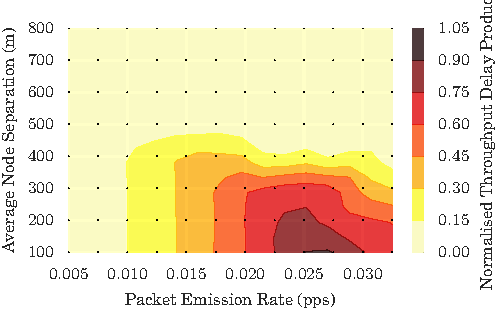
\includegraphics[width=\textwidth]{2d_normed_product_bella_all_mobile}
		\caption{All Mobile}
		\label{fig:2d_normed_product_bella_all_mobile}
	\end{subfigure}
	\caption{Normalised Throughput-Delay Product for all mobilities under varying separation and emission rate}
	\label{fig:2d_normed_product}
\end{figure}


\subsection{Summary}

An appropriate safe operating zone for marine communications has been established by investigating the impact of variations of the communications rate and physical distribution across the mobility scenarios.

These findings can be summaries as that when the separation is increased, the emission rate at which the network becomes saturated decreases, reducing overall throughput. 
This throughput degradation is tightly coupled with the mobility, as increasing mobility leads to increasing delays as routes are constantly broken, re-advertised and re-established. 
For instance, where all nodes are static, significant drops in throughput are not seen until node separation approaches $\SI{800}{\meter}$, nearly double the initial estimate. 
However, when all nodes are randomly walking the saturation point collapses from $0.025pps$ at $\SI{300}{\meter}$ to $0.015pps$ at $\SI{400}{\meter}$.\todo[inline]{FIX:Double Check These Saturation Points Before Release}
These results indicate that a good area to continue operating in for a range of node separations is at $0.015pps$, and that a reasonable position scaling is from $\SI{100}{\meter}$ to $\SI{300}{\meter}$, beyond which communication becomes increasingly unstable, especially in terms of end-to-end delay.
These results are similar to related simulation work \cite{Miquel2008,Diamant2010,Noh2012}, and is to be expected in such a sparse, noisy, and contentious environment.
It should be noted that these rates are not what would be expected in a single-node/single-operator environment that most current \gls{auv} operations inhabit, as without any channel contention and mixed-delay effects, data-rates many times higher than this would be expected.
However, few practical experiments have been performed that are suitable for direct comparison, as this context relies on multiple available nodes in a dynamic \gls{manet} topology with differential mobility.


\todo{ADD:expand this section to include discussion and results of single mobility models}
The results from \autoref{fig:2d_normed_product_bella_single_mobile} and \autoref{fig:2d_normed_product_bella_allbut1_mobile} show that the single-node differential mobility models don't capture the reality of the network in the proposed port-protection context.
The reason for this is that in these single-differential mobility combinations, the node targeted for misbehaviour ($n_1$) will already be behaving differently compared to the rest of the network regardless of the misbehaviour.
A future extension to this work could be to look at differential ratios of static/mobile nodes in alternative scenarios, such as in data-muling applications or \gls{wsn}.

\section{Operation of \glspl{tmf} in \glspl{uan}}

We are primarily concerned with the direct trust relationship between $n_0$ and $n_1$, i.e. $n_0$'s assessment of the trustworthiness of $n_1$, or $T_{1,0}$.

\citet{Guo11} introduce a range of misbehaviours, including modification of the packet loss rate of routing nodes and limiting throughput on a per-link basis as well as a selection of combined misbehaviours. 
\todo{FIX:Link back to intro/bg misbehaviour dicussion}
Given that the established links are already heavily constrained, such attacks would severely impact the general performance of the network beyond the scope of simple selfishness.
These direct malicious behaviours effectively trigger saturation collapses in operating regions of the network that should be stable.

Therefore, two more subtle misbehaviours to investigate are; 
\begin{enumerate}
	\item \acrfull{mpc}, where $n_1$ increases its transmit and forwarding power by 20\% for all nodes \emph{except} communications from $n_0$ in order to make $n_0$ appear to be selfishly conserving energy to the rest of the team, while $n_1$ itself appears to be performing very well.
	\item \acrfull{sts}, where $n_1$ preferentially communicates, forwards and advertises to nodes that are physically close to it in effort to reduce its own power consumption.
\end{enumerate}


\section{Simulation Results and Discussion}\label{sec:trustresultsanddiscussion}

Having established a safe operating range for comparison at $\SI{300}{\meter}$ average separation and an emission rate of $0.015pps$, each of the three selected behaviours (Fair, \gls{mpc}, \gls{sts}) are performed in both the static and mobile scenarios. 
We select a trust assessment period of 10 mins for a five hour mission to scale in comparison to relative bitrates experienced ($1Mbps$ vs $\approx15bps$).

The six metrics used for grey assessment are; transmitted and received throughput and power, delay, and \gls{plr} as calculated by aborted and unacknowledged, transmissions.
Compared to \cite{Guo11}, this metric set lacks a data rate quantity as the network is not dynamically adjusting bandwidth.
In context of \gls{grc} generation \eqref{eq:grc}, the best sequence $g$ was selected using the lowest \gls{plr}, delay, and powers, and the highest throughputs, and the worst sequence, $b$ the inverse of these metrics, reflecting the observations made in \autoref{sec:trust_in_marine}.

The particular factors under discussion are the relative performance of \gls{mtfm} against \gls{otmf} and Beta with respect to statistical stability across mobilities and in responsiveness to changing network behaviour. 
We establish a similar result set by initially tracking the resultant trust values established by \gls{mtfm} in the pair of mobility scenarios, shown in Fig.~\ref{fig:trust_mobility}.
We are also concerned with the opinions of $n_1$ provided to $n_0$ by other nodes, where $[T_{2,1},T_{3,1}]$ and $[T_{4,1},T_{5,1}]$ denote the sets of recommendation and indirect trust assessment respectively.

We also include aggregate assessments; $T_{N,1}^\text{Avg}$, the unweighted mean of direct trust assessments of $n_1$ from all nodes and $T_{0,1}^\text{MTFM}$, the final \gls{mtfm} trust assessment value based on both network topology with respect to $n_0$ and whitenization from \eqref{eq:whitenization}.

The variability in assessment is coupled to mobility; in the static case (Fig.~\ref{fig:trust_static}), the nodes exhibit relatively consistent distributions.
In the full mobility case, shown in Fig.~\ref{fig:trust_all_mobile}, this subjective variability is greatly increased. 
As the topology is highly dynamic, delays due to re-establishing routes can be very large, perturbing the trust value.
The $T_{0,1}^\text{MTFM}$ displays a significantly reduced variation than those of the individual subjective observations in all cases, even when compared to the unweighted average, $T_{N,1}^\text{Avg}$.
This demonstrates $T_{MTFM}$'s value as an aggregating trust assessment in such sparse and noisy environments.
Further, in Fig.~\ref{fig:trust_all_mobile_mal} a much higher variability in assessment is observed in $T_{0,1}$, correctly indicating that there is something wrong with the relationship between $n_0$ and $n_1$.

\begin{figure}[h]
	\centering
	\begin{subfigure}{0.5\textwidth}
		\caption{Fair Static}
		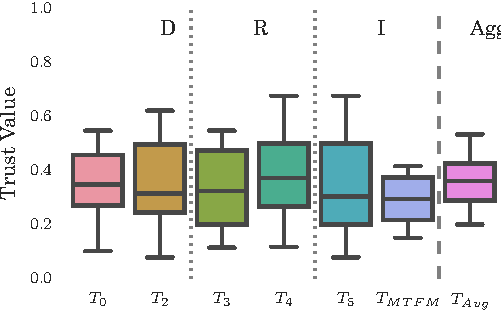
\includegraphics[width=\linewidth]{trust_bella_static_fair} 
		\label{fig:trust_static}
	\end{subfigure}%
	\begin{subfigure}{0.5\textwidth}
		\caption{Fair Mobile}
		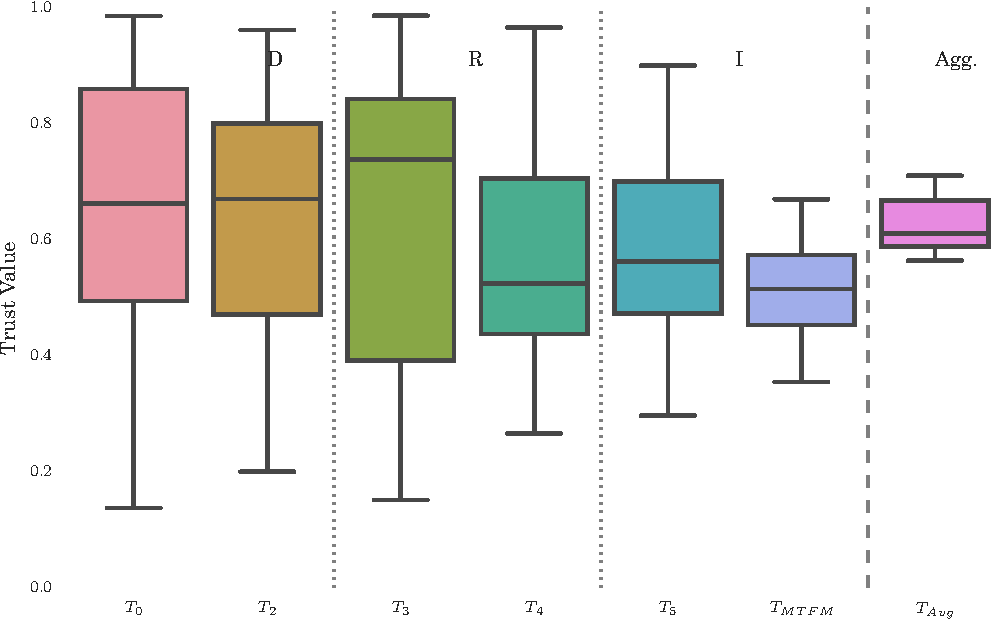
\includegraphics[width=\linewidth]{trust_bella_all_mobile_fair}  
		\label{fig:trust_all_mobile}
	\end{subfigure}%
	
	\begin{subfigure}{0.5\textwidth}
		\caption{Malicious (MPC) Static}
		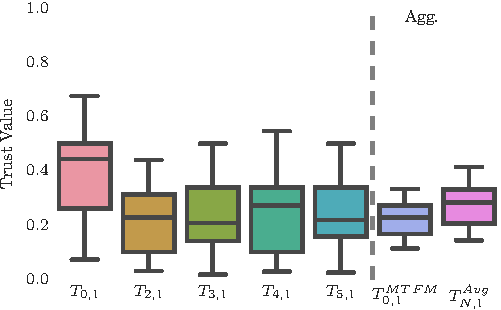
\includegraphics[width=\linewidth]{trust_bella_static_malicious} 
		\label{fig:trust_static_mal}
	\end{subfigure}%
	\begin{subfigure}{0.5\textwidth}
		\caption{Malicious (MPC) Mobile}
		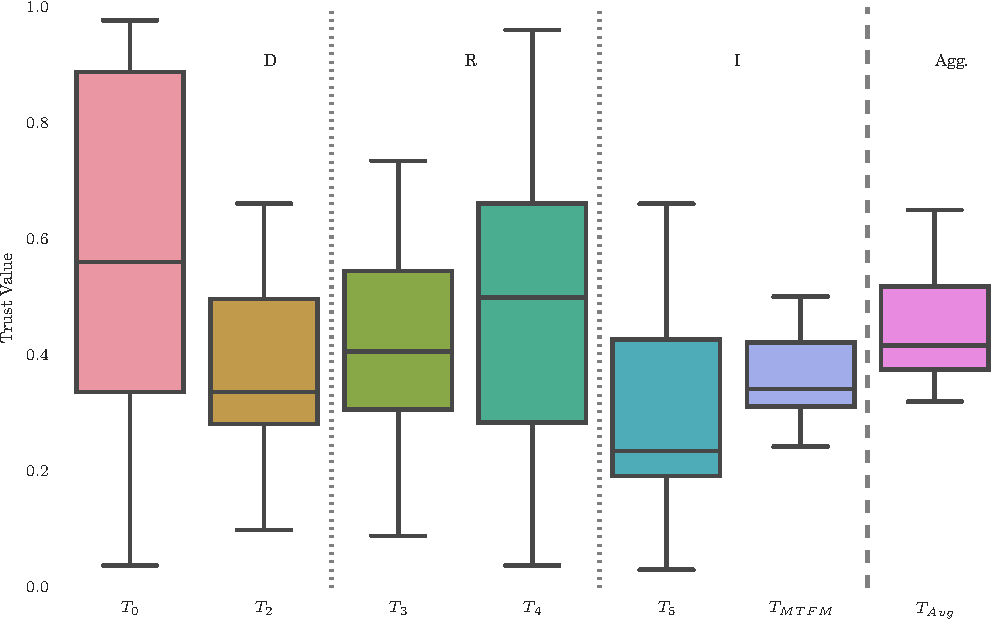
\includegraphics[width=\linewidth]{trust_bella_all_mobile_malicious}  
		\label{fig:trust_all_mobile_mal}
	\end{subfigure}%
	
	\begin{subfigure}{0.5\textwidth}
		\caption{Selfish (STS) Static}
		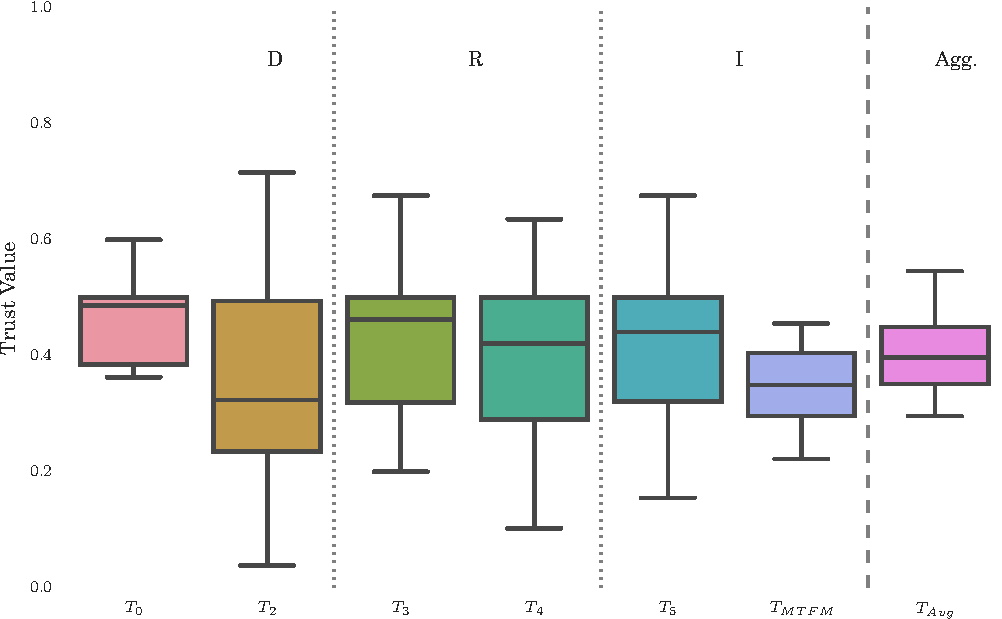
\includegraphics[width=\linewidth]{trust_bella_static_selfish}
		\label{fig:trust_static_sel}
	\end{subfigure}%
	\begin{subfigure}{0.5\textwidth}
		\caption{Selfish (STS) Mobile}
		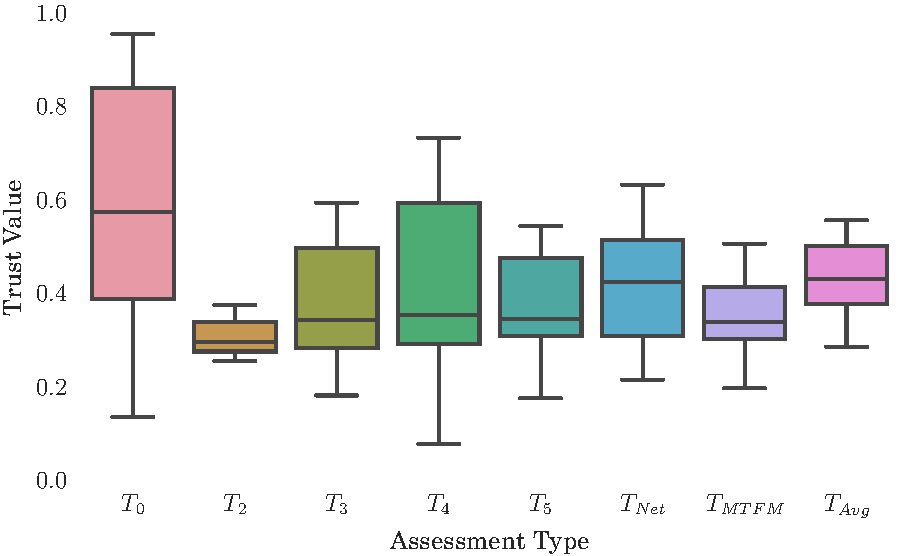
\includegraphics[width=\linewidth]{trust_bella_all_mobile_selfish}  \label{fig:trust_all_mobile_sel}
	\end{subfigure}%
	
	\caption{\gls{mtfm} Trust assessments of $n_1$ ($T_{X,1}$), showing Direct, Recommender and Indirect relationships, and derived aggregates} 
	\label{fig:trust_mobility}
\end{figure}
%

\subsection{Comparison between \gls{mtfm}, Hermes and \gls{otmf}}
As per \citet{Guo11}, ``fair'' scenarios were also performed with no malicious behaviour, applying \gls{otmf} and Hermes assessment as well as \gls{mtfm}, providing like-for-like comparison of assessment.

\begin{figure*}[t]
	\centering
	\begin{tabular}{cc}
		\multirow{2}{*}{
			\begin{subfigure}{0.45\textwidth}	
				\includegraphics[width=\linewidth]{trust_beta_otmf_fair}
				\caption{Fair Scenario}
				\label{fig:all_mobile_fair_beta}
			\end{subfigure}
		}&
		\begin{subfigure}{0.45\textwidth}
			\includegraphics[width=\linewidth]{trust_beta_otmf_malicious} 
			\caption{Malicious Power Control (MPC) Scenario}
			\label{fig:all_mobile_badmouthing_beta}
		\end{subfigure} \\
		&
		\begin{subfigure}{0.45\textwidth}	
			\includegraphics[width=\linewidth]{trust_beta_otmf_selfish} 
			\caption{Selfish Target Selection (STS) Scenario}
			\label{fig:all_mobile_selfish_beta}
		\end{subfigure}
	\end{tabular}
	\caption{$T_{0,1}$ for Hermes, \gls{otmf} and \gls{mtfm} assessment values for fair and malicious behaviours in the fully mobile scenario}
	\label{fig:otmf_beta_comparison}
\end{figure*}
%
\begin{figure}
	\centering
	\includegraphics[width=0.9\textwidth]{trust_beta_otmf_mtfm_boxes}
	\caption{Alternative Visualisation of \gls{tmf} performance comparison across Fair, \gls{mpc}, and \gls{sts} scenarios}
	\label{fig:otmf_beta_comparison_boxes}
\end{figure}
The use of \gls{fbr} and a \gls{csmaca} \gls{mac} scheme from AUVNetSim~\cite{Miquel2008} in our simulation mitigates a significant number of packet losses through collision avoidance and contention handling, leading to the situation that the only genuinely lost packets occur when a node moves completely out of range of any other node and time out occurs in route discovery rather than transmission (See \autoref{sec:manet_routing}).
As such, confirmed packet losses are relatively rare and in a delaying network like this, it is difficult to set a differentiating time out between packets that are in the network but queued, and packets that are actually ``lost''.

The single metric \glspl{tmf} used in conventional \gls{manet}s require regular and constant input to shape and adjust their evaluations, which for a network with significant and irregular delays such as this, is not practical.
This renders \gls{otmf} and Hermes assessment at best uninformative and at worst misleading; consistently providing nodes a high trust assessment as they have very little information to extract trust from. 

\autoref{fig:otmf_beta_comparison} shows a comparison between the unweighted response of \gls{mtfm} compared to \gls{otmf} and Hermes assessment functions on the same data for the fair, malicious and selfish behaviours respectively.
This time-series perspective demonstrates how noisy and variable the assessments from all \glspl{tmf} in this environment.
For clarity, \autoref{fig:otmf_beta_comparison_boxes} displays a compressed-time perspective, showing the overall trend and sensitivity of the different frameworks in the same scenarios as shown in \autoref{fig:otmf_beta_comparison}.
It is important to note a distinction between the expectations of \gls{mtfm} compared to other \glspl{tmf}; \gls{mtfm} is primarily concerned with the identification of differences in the behaviours of nodes in a network, and is relative rather than absolute.
That is to say that under \gls{mtfm}, nodes are compared against the worst current performances across metrics of other observed nodes and graded against them, rather than the absolute (objective) approach taken by many \glspl{tmf}.

In the case of the \gls{mpc}
In these cases, particularly since the methods of attack were not directly related to \gls{plr}, \gls{otmf} and Hermes have not registered significant activity in either misbehaviour when compared to the fair scenario.
The difference between the \gls{mtfm} trust assessments under ``fair'' and ``malicious'' behaviour is lowered by $\approx 10\%$ in both cases, in terms of the mean values returned.
At run time, similar results could be attained by an \gls{ewma}.

On their own, neither \gls{otmf}, Hermes, or unbiased \gls{mtfm} appear to be effective in detecting or identifying malicious behaviour in this environment, in fact \gls{otmf} and Hermes don't appear to differentiate between fair and selfish scenarios at all.



\subsection{Metric Vector Weighting}\label{sec:metric_weighting}
%

A sequence of vectors that preferentially weight each metric in \eqref{eq:metric_weighting} to each of the three simulation runs.
For a metric weight vector $H$, where the metric $m_j$ is emphasised as being twice as important as the other metrics, forming an initial weighting vector $H'=[h_i\dots h_M]$ such that $h_i = 1 \forall i \ne j; h_j=2$.
That vector $H'$ is normalised such that $\sum H = 1$ by $H= \frac{H'}{\sum H'}$.
Using this process the primary aspects of an attack can be extracted and highlighted by comparing against the deviation from the ``fair'' result set. 

\begin{figure}[h]
	\centering
	\begin{subfigure}{0.45\textwidth}
		\includegraphics[width=\linewidth]{trust_bella_all_mobile_emph_ADelay_BadMouthingPowerControl} 
		\caption{$\text{Delay}$ Emphasised}
		\label{fig:all_mobile_badmouthing_delay}
	\end{subfigure}
	\begin{subfigure}{0.45\textwidth}
		\includegraphics[width=\linewidth]{trust_bella_all_mobile_emph_PLR_BadMouthingPowerControl} 
		\caption{$PLR$ Emphasised}
		\label{fig:all_mobile_badmouthing_plr}
	\end{subfigure}
	
	\begin{subfigure}{0.45\textwidth}
		\includegraphics[width=\linewidth]{trust_bella_all_mobile_emph_ARXP_BadMouthingPowerControl} 
		\caption{Received Power ($P_{RX}$) Emphasised}
		\label{fig:all_mobile_badmouthing_rxp}
	\end{subfigure}	
	\begin{subfigure}{0.45\textwidth}
		\includegraphics[width=\linewidth]{trust_bella_all_mobile_emph_ATXP_BadMouthingPowerControl} 
		\caption{Transmit Power ($P_{TX}$) Emphasised}
		\label{fig:all_mobile_badmouthing_txp}
	\end{subfigure}
	
	\begin{subfigure}{0.45\textwidth}
		\includegraphics[width=\linewidth]{trust_bella_all_mobile_emph_RXThroughput_BadMouthingPowerControl} 
		\caption{Throughput ($S$) Emphasised}
		\label{fig:all_mobile_badmouthing_rxthroughput}
	\end{subfigure}
	\begin{subfigure}{0.45\textwidth}
		\includegraphics[width=\linewidth]{trust_bella_all_mobile_emph_TXThroughput_BadMouthingPowerControl} 
		\caption{Offered Load ($G$) Emphasised}
		\label{fig:all_mobile_badmouthing_txthroughput}
	\end{subfigure}
	\caption{$T_{1,0}^\text{MTFM}$ in the All Mobile case for the Malicious Power Control behaviour, including dashed $\pm\sigma$ envelope about the fair scenario}
	\label{fig:all_mobile_badmouthing}
\end{figure}
%
\begin{figure}[h]
	\centering
	\begin{subfigure}{0.45\textwidth}	
		\includegraphics[width=\linewidth]{trust_bella_all_mobile_emph_ADelay_SelfishTargetSelection} 
		\caption{$Delay$ Emphasised}
		\label{fig:all_mobile_selfish_delay}
	\end{subfigure}
	\begin{subfigure}{0.45\textwidth}	
		\includegraphics[width=\linewidth]{trust_bella_all_mobile_emph_PLR_SelfishTargetSelection}
		\caption{$PLR$ Emphasised}
		\label{fig:all_mobile_selfish_plr}
	\end{subfigure}
	
	\begin{subfigure}{0.45\textwidth}	
		\includegraphics[width=\linewidth]{trust_bella_all_mobile_emph_ARXP_SelfishTargetSelection}
		\caption{Received Power ($P_{RX}$) Emphasised}
		\label{fig:all_mobile_selfish_rxp}
	\end{subfigure}
	\begin{subfigure}{0.45\textwidth}
		\includegraphics[width=\linewidth]{trust_bella_all_mobile_emph_ATXP_SelfishTargetSelection}
		\caption{Transmit Power ($P_{TX}$) Emphasised}
		\label{fig:all_mobile_selfish_txp}
	\end{subfigure}
	
	\begin{subfigure}{0.45\textwidth}
		\includegraphics[width=\linewidth]{trust_bella_all_mobile_emph_RXThroughput_SelfishTargetSelection} 
		\caption{Throughput ($S$) Emphasised}
		\label{fig:all_mobile_selfish_rxthroughput}
	\end{subfigure}
	\begin{subfigure}{0.45\textwidth}
		\includegraphics[width=\linewidth]{trust_bella_all_mobile_emph_TXThroughput_SelfishTargetSelection} 
		\caption{Offered Load ($G$) Emphasised}
		\label{fig:all_mobile_selfish_txthroughput}
	\end{subfigure}
	\caption{$T_{1,0}^\text{MTFM}$ in the All Mobile case for the Selfish Target Selection behaviour, including dashed $\pm\sigma$ envelope about the fair scenario}
	\label{fig:all_mobile_selfish}
\end{figure}


Fig.~\ref{fig:all_mobile_badmouthing} shows that the malicious node is consistently outside the $\pm\sigma$ (one standard deviation above and below the mean) envelope of the fair scenario it's being compared to.
This is particularly true for \gls{plr}, with smaller impacts on delay, received power and offered load. 
This weighted delta in received throughput is minimal to insignificant compared to the width of the detection envelope, occasionally breaching the envelope for a short period. 

In the selfish case (Fig.~\ref{fig:all_mobile_selfish}) a much lower weighted delta in \gls{plr} and delay is observed, with greatly increased impact on transmission power.
In comparison to \cite{Guo11}, these results are qualitatively similar, however here the differences between the fair case and the misbehaviours are less clear than in the comparable terrestrial space.
\citet{Guo11} show similar types of behaviour but report a weighted delta from $\approx$ 0.4 to $\approx$ 0.9 across the simulation period, compared to our maximum delta in $P_{TX}$ in selfish behaviour (Fig.~\ref{fig:all_mobile_selfish_txp}) of $\approx$ 0.3 for an inconsistent interval.

\subsection{Weight Significance Analysis for Behaviour Classification}

For a more quantitative assessment of the viability of multi-metric trust assessment methods, taking the qualitative analysis above and apply a Random Forest regression \cite{Breiman2001} to assess the relative importance of the selected metrics on relative detectability of malicious behaviour. 
Random Forest accomplishes this by generating a large number of random regression trees and prunes these trees to fit incoming data.
The target function for this regression was the area between the target behaviours weighted $T_{MTFM}$ curve and the $\pm\sigma$ envelope of the base behaviour as shaded in Figs.~\ref{fig:all_mobile_badmouthing} and~\ref{fig:all_mobile_selfish}.
From this training process, the relative importance of each input feature (metric) can be inferred in terms of how good it is to differentiate between the fair case and a given misbehaviour.
Additionally a cross correlation analysis is performed to establish the correlations between given metric weighting emphasis and the output of the target function.
Our intention is to establish the metrics that not only differentiate both misbehaviours from the fair case, but also what metrics differentiate the two misbehaviours from each other.

Applying this target regression to 729 different metric weight vector emphasis combinations reveals that each of the three combinations (i.e.\ comparing fair to misbehaviours, and comparing the misbehaviours) present distinct patterns of significance in three primary metrics; received throughput, transmitted power, and PLR, with delay, received power and transmitted throughput playing a lesser role.
Practically this means that in order to accurately distinguish between these scenarios, these primary metrics should be higher-weighted in the generation of $T_{1,MTFM}$ in \eqref{eq:networkeffects}.

It may initially appear odd that the relative significance of the received throughput is similar between all three scenario combinations, however a correlation analysis shows that in the MPC attack; the received throughput is positively correlated with successful classification against the fair case ($R=+0.71, p\approx10^{-100}$), while the inverse is the case for the STS attack ($R=-0.70, p\approx10^{-100}$).
It is expected that Transmitted power should be the defining characteristic of STS ($R=+0.72, p<10^{-100}$) as the node is acting fairly from a protocol perspective but is acting unfairly at a higher (incentive) level; it is performing fairly in terms of it's communications with other nodes, however it is preferring to communicate with nodes that it can expend less energy communicating with.
A summary of these correlations is shown in Table.~\ref{tab:correlations}.

Comparing Figs.~\ref{fig:otmf_beta_comparison},~\ref{fig:all_mobile_badmouthing_plr}, and~\ref{fig:all_mobile_selfish_plr}, while it is possible that in a cleaner, less sparse, and less noisy environment, \gls{otmf} would be able to detect the \gls{mpc} behaviour, Fig.~\ref{fig:malselfactors} shows that \gls{plr} plays almost no part at all in detecting the \gls{sts} behaviour, and so \gls{otmf} would not detect the attack.

\begin{figure}
	\centering
	\includegraphics[width=0.95\linewidth]{MaliciousSelfishMetricFactors}
	\caption{Random Forest Factor Analysis of Malicious (\gls{mpc}, Selfish (\gls{sts}) and Fair behaviours compared against each-other}
	\label{fig:malselfactors}
\end{figure}

\begin{table}[h]
	\caption{Correlation Coefficients between metric weights and behaviour detection targets} \label{tab:correlations}
	\begin{center}
		\begin{tabular}{lcccccc}
			\toprule
			Correlation      & Delay & $P_{RX}$ & $P_{TX}$ & $G$ & $S$ & PLR \\
			\midrule
			Fair / MPC       & 0.199 &  0.159   & -0.416  &  0.708   & -0.238   & -0.401\\
			Fair / STS       & 0.179 &  -0.009  &  0.724  & -0.697   & -0.145   & -0.052\\
			MPC / STS        & 0.058 &  -0.134  &  0.146  & -0.768   &  0.052   &  0.146\\
			\bottomrule
		\end{tabular}
	\end{center}
\end{table}

As such this presents the open opportunity to develop a heuristic weight search scheme to detect malicious behaviour without the comparison to the fair scenario.
This would be accomplished by assessing the impact of differential metric weighting on the mean trust assessment rather than comparing co-weighted valuations across scenarios.

\section{Conclusion}
It has been demonstrated that existing \gls{manet} Trust Management Frameworks are not directly suitable to the sparse, noisy, and dynamic underwater medium.
By comparing the operation and performance of trust establishment in \glspl{manet} in a simulated underwater environment has demonstrated that in order to have any reasonable expectation of performance, that throughput and delay responses must be characterised before implementing trust. 
While the \gls{mtfm} value does not display any immediate difference between the two behaviours, it has been shown that by exploring the metric space by weight variation, the existence and nature of the malicious behaviour can be discovered.
Another difference is that \gls{mtfm} is significantly more computationally intensive than the relatively simple Hermes / \gls{otmf} algorithms.
The repeated metric re-weighting required for real time behaviour detection is therefore an area that requires optimization.
With significant delays (from seconds to many minutes), in a fading, refractive medium with varying propagation characteristics, the environment is not as predictable or performant as classical \gls{manet} \gls{tmf} deployment environments.

It is shown that, without significant adaptation, single metric probabilistic estimation based \glspl{tmf} are ineffective in such an environment.
Additionally, it's clear that existing frameworks are overly optimistic about the nature and stability of the communications channel, and can overlook characteristics that are useful for assessing the behaviour of nodes in the network. 
This indicates that there is a good case, particularly within constrained \gls{manet}Ìs as this, for multi-vector, and even multi-domain trust assessment, where metrics about the communications network and topology would be brought together with information about the physical behaviours and operations of nodes to assess trust.

A significant additional factor of trust assessment in such a constrained environment is that there may be long periods where two edge nodes (for instance, $n_0 \to n_5$) may not interact at all. 
This can be due to a range of factors beyond malicious behaviour, including simple random scheduling coincidence and intermediate or neighbouring nodes collectively causing long back-off or contention periods.
This disconnection hinders trust assessment in two ways; assessing nodes that do not receive timely recommendations may make decisions based on very old data, and malicious nodes have a long dwelling time where they can operate under a reasonable certainty that the \gls{tmf} will not detect it (especially if the node itself is behaving disruptively).

However the demonstrated noisiness and sparseness of communications metrics for trust assessment indicate that it may be more beneficial to look to other domains beyond communications to establish trust, such as the physical domain where we are concerned with the motion, placement and behaviour of the network nodes.


%%%%%%%%%%%%%%%%%%%%%%%%%%%%%%%%%%%%%%%%%%%%%%%%%%%%%%%%%%%%%%%%%%%%%%%%%%%%%%%
